%%%%%%%%%%%%%%%%%%%%%%%%%%%%%%%%%%%%%%%%%%%%%%%%%%%%%%%%%%%
%                                                         %
%       This is documentation for the IFJ project.        %
%                                                         %
%%%%%%%%%%%%%%%%%%%%%%%%%%%%%%%%%%%%%%%%%%%%%%%%%%%%%%%%%%%


%------------------------------------------------%
%	    CONFIGURATION + IMPORTED PACKAGES        %
%------------------------------------------------%
\documentclass[12pt,a4paper,titlepage]{report}
\usepackage[english]{babel}
\usepackage[utf8]{inputenc}
\newcommand\HRule{\rule{\textwidth}{1,5pt}}

\usepackage{titlesec}
\usepackage{geometry}   % paper size
 \geometry{
 a4paper,
 total={160mm,255mm},
 left=25mm,
 top=25mm,
 bottom=25mm
 }

\titleformat{\chapter}{\Huge\bfseries}{}{0pt}{\Huge\bfseries}   % chapters space
\titlespacing*{\chapter}{0pt}{-32pt}{23pt}

\usepackage{tikz}       % Borders
\usetikzlibrary{calc}

\usepackage{graphicx}   % Import pictures

\usepackage{wrapfig}    % pictures between paragraphs
\usepackage{ragged2e}   % fullfill paragraphs

\usepackage{blindtext}   % text generator

\begin{document}
%-----------------------------------------%
%	            TITLE PAGE                %
%-----------------------------------------%
\begin{titlepage}


\begin{tikzpicture}[overlay,remember picture]       % Borders around title page

    \draw [line width=1pt,rounded corners=7pt]
    ($ (current page.north west) + (0.65cm,-0.65cm) $)
    rectangle
    ($ (current page.south east) + (-0.65cm,0.65cm) $);

    \draw [densely dotted,line width=0.75pt,rounded corners=7pt]
    ($ (current page.north west) + (1.15cm,-1.15cm) $)
    rectangle
    ($ (current page.south east) + (-1.15cm,1.15cm) $);

        %\draw [line width=1pt,rounded corners=7pt]
        %($ (current page.north west) + (1.5cm,-1.5cm) $)
        %rectangle
        %($ (current page.south east) + (-1.5cm,1.5cm) $);

\end{tikzpicture}



\begin{center}

% Headings
\textsc{\LARGE Brno University of technology}\\[1.5cm]

\textsc{\large Faculty of Information Technology}\\[3cm]

% Title - lines
\HRule \\[0.5cm]
{ \Huge \bfseries IFJ project}\\[0.3cm]
{ \large \bfseries documentation}\\[0.4cm]
{ \normalsize \bfseries 2017}\\[0.1cm]
\HRule \\[2.3cm]

\end{center}


% Table of authors
\begin{center}
    \begin{tabular}{ll}
    \multicolumn{2}{l}{\hspace{45pt} \large \underline{Authors}} \\
                                 \\
    Martin Beneš      & xbenes49 \\
    Ksenia Bolshakova & xbolsh00 \\
    Petr Kratochvíl   & xkrato47 \\
    Ondřej Polanský   & xpolan09 \\
    \end{tabular}
\end{center}


%\begin{tabular}[t]{@{}l@{\hspace{5pt}}p{.52\textwidth}@{}}
%Authors: \\
%& Martin Beneš      \hspace*{0.49in}xbenes49 \\
%& Ksenia Bolshakova \hspace*{0.49in}xbolsh00 \\
%& Petr Kratochvíl   \hspace*{0.49in}xkrato47 \\
%& Ondřej Polanský   \hspace*{0.49in}xpolan09
%\end{tabular}

\vspace{3.0cm}

\begin{center}
\normalsize Brno,\\
{\normalsize\today} % Date
\end{center}

\newpage
\end{titlepage}


%-----------------------------------------%
%	         TABLE OF CONTENTS            %
%-----------------------------------------%

\tableofcontents  % The table of contents
\thispagestyle{empty}
\newpage


%-----------------------------------------%
%	            CHAPTERS                  %
%-----------------------------------------%

%\setcounter{page}{1}
%\pagenumbering{arabic}

\chapter*{Lexical analyse}                                            %%% -1- %%%
\addcontentsline{toc}{chapter}{Scaner}
    \section{Intro}

\begin{justify}
We did the scanner in two ways: singlethread and multithread work. Both variants work on the basis of the State Automaton.
The state machine was created on the basis of regular expression designs for individual types of phrases: cel number, decimal number with decimal point and positive or negative exponent, string, operator, identifier, keyword, commentary.\justify
Regular prints for:
of these regulars finally came into being.\justify

Singlethread is done as a common feature, multithread is done in a separate thread.\justify

For the purpose of decomposition, the structure of the lexical analyzer was divided into several subprograms that implemented individual parts.
\end{justify}

\begin{justify}
Numerals, decimal numerals, exponential numbers are given in function \textbf{getNumber}
\end{justify}

%(pick # getNumber)
\vspace{0.3cm}

\begin{wrapfigure}{r}{1.0\textwidth}
  \begin{center}
    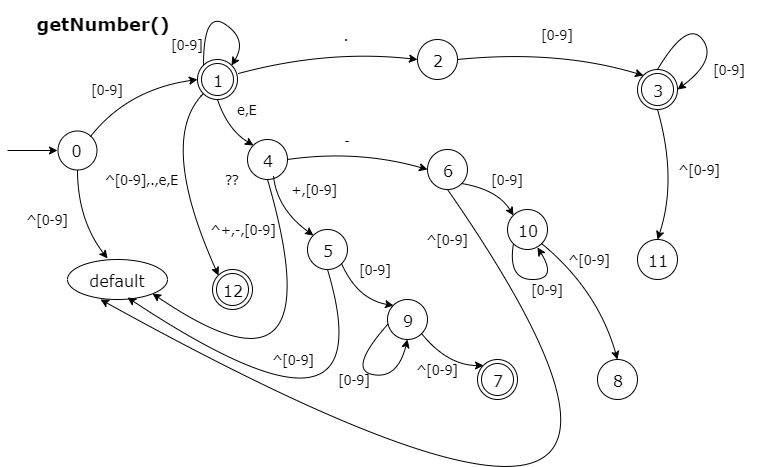
\includegraphics[width=1.0\textwidth]{img/getNumber.png}
  \end{center}
  %\caption{get}
\end{wrapfigure}

%\vspace{0.4cm}
%%%

\begin{justify}
String from \textbf{getString}
\end{justify}

%(pic # getString)
%\vspace{0.3cm}

\begin{wrapfigure}{r}{1.0\textwidth}
  \begin{center}
    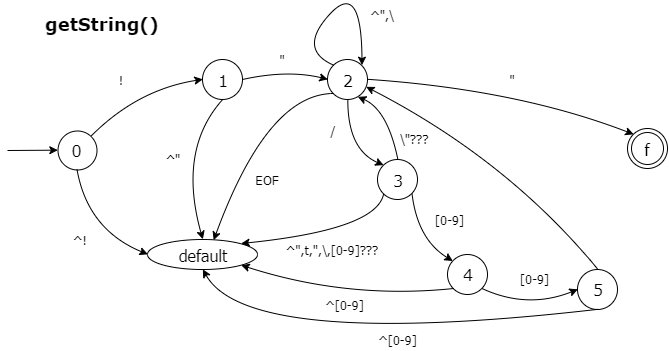
\includegraphics[width=1.0\textwidth]{img/getString.png}
  \end{center}
  %\caption{get}
\end{wrapfigure}

%\vspace{0.4cm}
%%%

\begin{justify}
The comment is in the \textbf{getComment} function.
There we resolved the problem with one "/" or "//", we resolved it by replacing "//" tilda ~ ".
\end{justify}

%%%(pic # getComment)
\vspace{0.3cm}

\begin{wrapfigure}{r}{1.0\textwidth}
  \begin{center}
    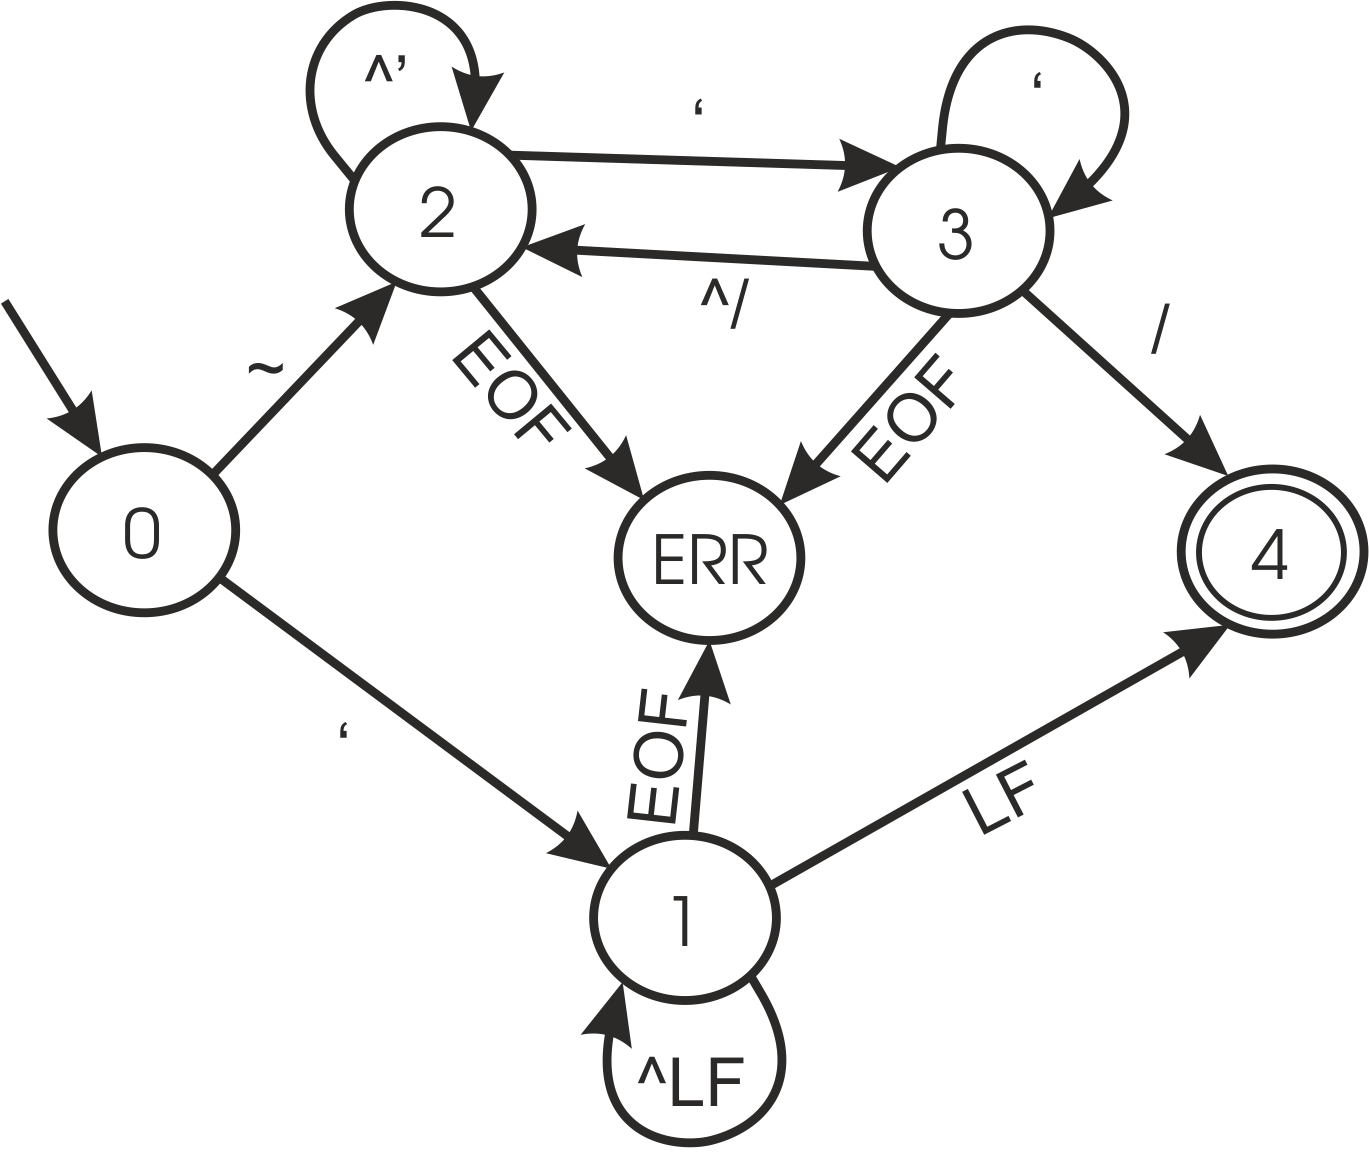
\includegraphics[width=1.0\textwidth]{img/getComment.png}
  \end{center}
  %\caption{get}
\end{wrapfigure}

\vspace{0.4cm}
%%%

\begin{justify}
Identifiers and keyword words are rendered in the \textbf{getIdentifier} function
\end{justify}

%(pic # get Identifier)
\vspace{0.3cm}

\begin{wrapfigure}{r}{1.0\textwidth}
  \begin{center}
    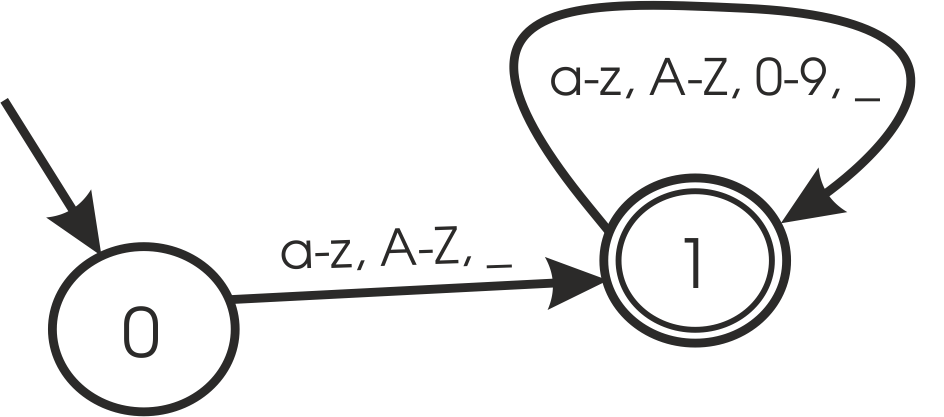
\includegraphics[width=1.0\textwidth]{img/getIdentifier.png}
  \end{center}
  %\caption{get}
\end{wrapfigure}

\vspace{0.4cm}
%%%

\begin{justify}
Operators are processed in \textbf{getOperator}
\end{justify}

%(pic # getOperator)
\vspace{0.3cm}

\begin{wrapfigure}{r}{1.0\textwidth}
  \begin{center}
    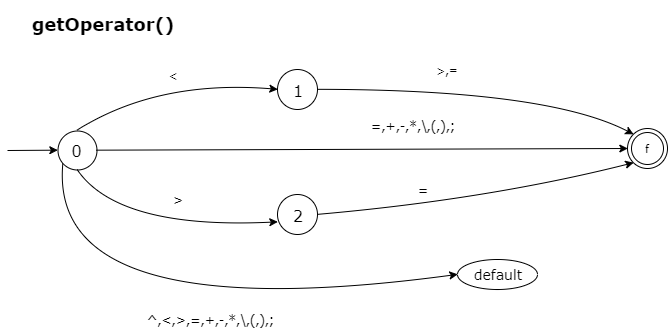
\includegraphics[width=1.0\textwidth]{img/getOperator.png}
  \end{center}
  %\caption{getOperator}
\end{wrapfigure}

\vspace{0.4cm}
%%%


\begin{justify}
For the sake of implementation, we put the wrapper over the input to return the character back to the input. The function is called \textbf{returnByte()}.
\end{justify}



% ------------------------------------------------------- %

\iffalse

\chapter*{Pars..}                                                       %%% -2- %%%
\addcontentsline{toc}{chapter}{Parser}
    \section{Intro}
    \Blindtext

\fi

\end{document}
